\documentclass[a4paper,12pt,russian]{article} %draft
\usepackage[T2A]{fontenc}% Поддержка русских букв


% XeTeX packages
\usepackage[cm-default]{fontspec} % or install lmodern and remove cm-default opt
\usepackage{xunicode} % some extra unicode support
\usepackage{xltxtra} % \XeLaTeX macro


\tolerance=1000
\emergencystretch=0.74cm
\usepackage{indentfirst} %делать отступ в начале параграфа

\usepackage[pdfborder = {0 0 0}]{hyperref} %гиперссылки в документе.

\usepackage[utf8]{inputenc}	% кодировка текста
\usepackage[russian]{babel}	% руссификация по Бабелю
\usepackage{graphics}

\usepackage[clean,pdf]{svg}

\usepackage{amsmath, amsfonts} % для расширенных настроек ссылок на формулы
\usepackage{extsizes}	% использование шрифтов большего кегля
\usepackage{fancyvrb} % Добавляет продвинутые Verbatim и Verb

\usepackage{epsfig} % удобно вставлять рисунки в строку текста
\usepackage[usenames,dvipsnames]{pstricks}
\usepackage{pst-grad} % For gradients
\usepackage{pst-plot} % For axes

\usepackage{graphicx,xcolor}

%\usepackage[MakeStamp]{eskdi}
%\usepackage[MakeStamp, SubSectInToc]{eskdi}
%\usepackage[MakeStamp, SubSubSectInToc]{eskdi}
%\usepackage[MakeStamp, ParagraphInToc]{eskdi}
%\usepackage[twoside, MakeStamp, ParagraphInToc]{eskdi}
%\usepackage{eskdi}
%\usepackage[SubSectInToc]{eskdi}
%\usepackage[SubSubSectInToc]{eskdi}
%\usepackage[ParagraphInToc]{eskdi}
%\usepackage[ParagraphInToc, NumIntoSections]{eskdi}
%\usepackage[twoside, ParagraphInToc]{eskdi}
%\usepackage[twoside, MakeEmptyStamp, ParagraphInToc]{eskdi}
\usepackage[twoside, MakeEmptyStamp]{eskdi}
%\usepackage[MakeEmptyStamp, ParagraphInToc]{eskdi}



\usepackage{array}
\usepackage{tabularx}
\usepackage{supertabular}
\usepackage{longtable} % для создания таблиц, переносящихся на другую страницу
%\usepackage{listingsutf8}%
\usepackage{listings} % для включения листинга кода в приложения. Русский язык глючит.


\lstloadlanguages{bash,[LaTeX]TeX,MetaPost,Clean,Matlab}


\usepackage{textcomp}	% Ввод различных знаков
\usepackage{keystroke} % для отображения символов клавиш
\usepackage{bytefield} %для создания таблиц с битовыми полями
\usepackage{filecontents} %для включения в документ содержимого файлов

\usepackage{tikz} % Пакет для рмсования диаграмм
\usepackage{tikz-timing}[2009/12/09]
\usetikzlibrary{positioning,arrows,automata,plotmarks} %В данном случае нам потребуются positioning и arrows, которые нужны для расположения элементов друг относительно друга и рисования стрелок между ними соответственно.
\usetikzlibrary{shapes,snakes}
\usepackage{schemabloc}

\usepackage{makecell} % Для многострочных ячеек таблицы
\usepackage{colortbl} % Для раскрашивания ячеек в таблицах


%{Arial} {Courier New} 
%{OpenGost Type A TT} {OpenGost Type B TT} % Свободный шрифт. Нет наклонного начертания и дирного начертания
%{GOST type A} % Морально устарел, не свободный, не хватает символа тирэ. Не рекомендуется
%{GOST type B} % Морально устарел, не свободный, не хватает символа тирэ. Не рекомендуется
\gostSetRomanfont{Times New Roman}%
\gostSetSansfont{Times New Roman}%
\gostSetMonofont{Times New Roman}%
\gostSetMainfont{Times New Roman}%
\gostSetStampfont{Arial}%


%\verbatimfont{\fontspec[Scale=1.0]{Arial} \itshape}% % Для замены стиля начертания verbatim и verb
\verbatimfont{\fontspec[Scale=1.0]{Consolas}}% % Для замены стиля начертания verbatim и verb
\newfontfamily{\gostListingfont}[Scale=1.0]{Consolas} % Шрифт для листингов
%\renewcommand{\SetStampfontIt}{\itshape}%

%\input commands.tex %Файл включает такие команды как надчёркивание, запрещение переноса ТУ и др.
\setpage % Разметка текста на странице
\begin{document}

	\gosttitleobject{Лабораторная работа}
		
	\gosttitledocument{ИССЛЕДОВАНИЕ МАТЕМАТИЧЕСКОЙ МОДЕЛИ ЭЛЕКТРОМЕХАНИЧЕСКОГО ОБЪЕКТА УПРАВЛЕНИЯ}

	% Раскомментировать если необходима утверждающая надпись на титульном листе
	\renewcommand\titleBotRIGHT{
	\spboxmm{100}{70}{70}{30}{lc}{\parbox{70mm}{
			\normalsize{Преподаватель: Чепинский С.А. }\\ 
			\normalsize{Студенты: Французов Р.А.\\  Донцова М.А.}\\
			\normalsize{Группа: R3325}\\
			\normalsize{Вариант: 18}}}}

		\maketitle
		
		\section{Цель работы}
Изучение математических моделей и исследование характеристик
электромеханического объекта управления (ЭМО), построенного на основе электродвигателя
постоянного тока независимого возбуждения. \\
		
		\section{Ход работы}
В программном пакете $SciLab$ $XCos$ были созданны полная (рис. \ref{p1}) и упрощенная (рис. \ref{p7}) структурные модели ЭМО, промоделированы переходные процессы при различных значениях параметров \\


\subsection{Расчет параметров}
В таблице ниже представлены начальные и расчитанные параметры модели
\begin{center}
	\begin{tabular}{|c|c|c|}
		\hline
		$U_n$ & &27 V\\ \hline$n_0$ & &6500 rpm\\ \hline$I_n$ & &0.92 A\\ \hline$M_n$ & &0.12 Nm\\ \hline$R$ & &16.6 $\Omega$\\ \hline$T_a$ & &7 ms\\ \hline$J_m$ & &0.00007 $kgm^2$\\ \hline$T_y$ & &4 ms\\ \hline$i$ & &50 \\ \hline$J_l$ & &0.01 $kgm^2$\\ \hline$\omega_0$ & $n_o/10&$650 rad/s\\ \hline$K_m$ & $1/R&$0.060241 \\ \hline$K_y$ & $U_n/10&$2.7 \\ \hline$K_m$ & $M_n/I_n&$0.060241 \\ \hline$J_r$ & $0.2J_m&$0.000014$kgm^2$ \\ \hline$k_1=k_e$ & $U_n/\omega_0$&0.0415385 \\ \hline$k_2=k_m$ & $M_n/I_n&0.1304348 \\ \hline$J_\Sigma$ &$J_m+J_r+\dfrac{J_l}{i^2} $&0.000088 \\ \hline$K$ & $\dfrac{K_y}{iK_e}$&1.3 \\ \hline$K_f$ & $\dfrac{R}{K_m K_e i^2}$&1.2255309 \\ \hline$T_m$ & $\dfrac{R J_\Sigma}{K_m K_e}$&0.2696168 ms\\ \hline

	\end{tabular}
\end{center}

\begin{figure}[H]
	\centering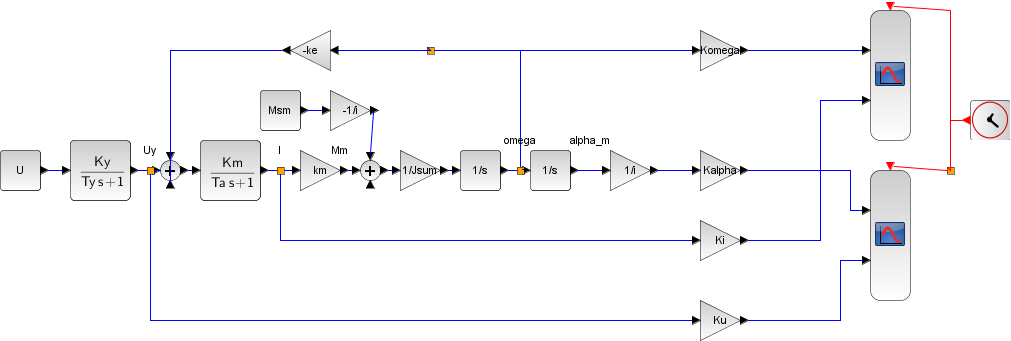
\includegraphics[width=0.9\textwidth]{1.png}
	\caption{Полная структурная модель ЭМО}\label{p1}
\end{figure}

\subsection{Первичное моделирование}
Ниже представлены переходные процессы  $\alpha\:  U_y$ (рис \ref{p21}) и $\omega\:  I$ (рис \ref{p22})  при  $U=5\: M_{sm}=0$.

\begin{figure}[H]
	\minipage{0.5\textwidth}
		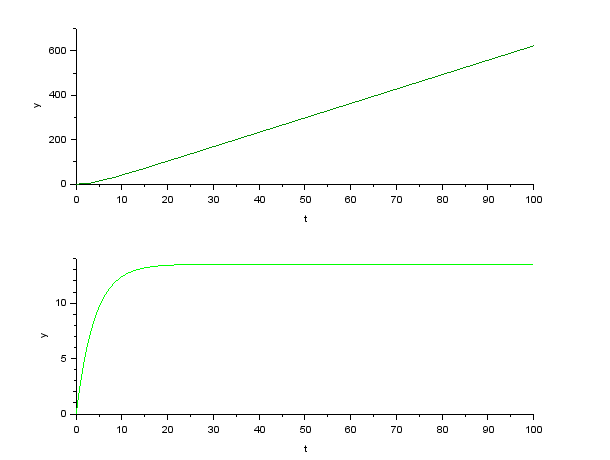
\includegraphics[width=\linewidth]{21.png}
		\caption{Переходные процессы $\alpha\:  U_y$}\label{p21}
	\endminipage\hfill
	\minipage{0.5\textwidth}
		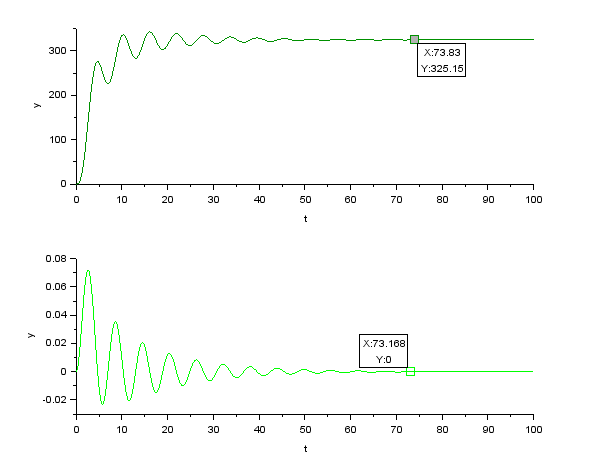
\includegraphics[width=\linewidth]{22.png}
		\caption{Переходные процессы $\omega\:  I$}\label{p22}
	\endminipage
\end{figure}

\subsection{Моделирование с различным моментом сопротивления}
Ниже представлены переходные процессы:\\
\begin{enumerate}
	\item  $\alpha\:  U_y$ (рис \ref{p311}) и $\omega\:  I$ (рис \ref{p312})  при  $U=5\: M_{sm}=\dfrac{iM_n}{2}=300Nm$
	\item  $\alpha\:  U_y$ (рис \ref{p321}) и $\omega\:  I$ (рис \ref{p322})  при  $U=5\: M_{sm}=iM_n=600Nm$
\end{enumerate} 

\begin{figure}[H]
	\minipage{0.5\textwidth}
	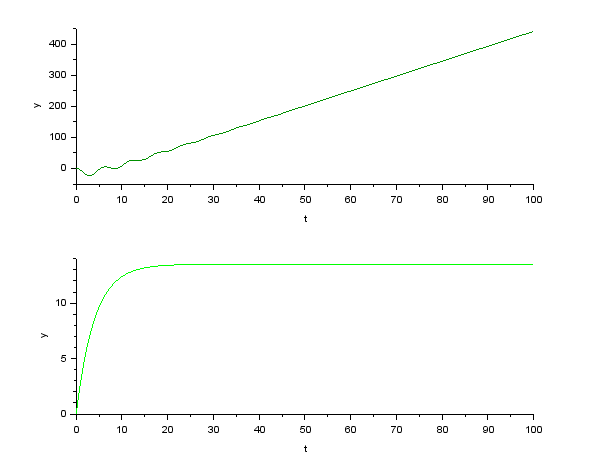
\includegraphics[width=\linewidth]{311.png}
	\caption{Переходные процессы $\alpha\:  U_y$}\label{p311}
	\endminipage\hfill
	\minipage{0.5\textwidth}
	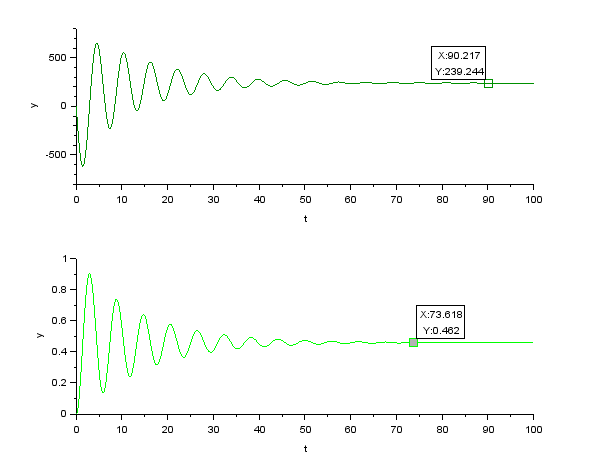
\includegraphics[width=\linewidth]{312.png}
	\caption{Переходные процессы $\omega\:  I$}\label{p312}
	\endminipage
\end{figure}
\begin{figure}[H]
	\minipage{0.5\textwidth}
	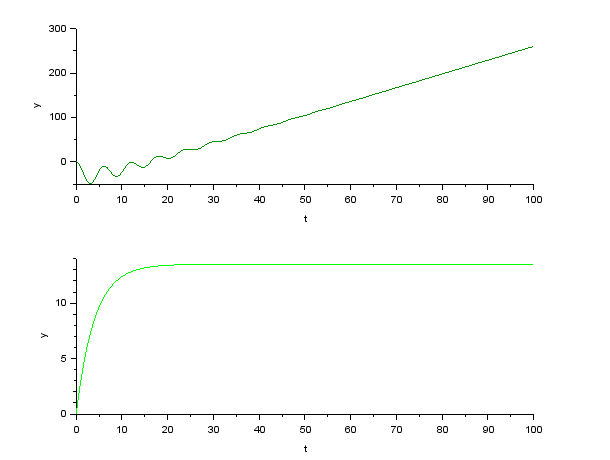
\includegraphics[width=\linewidth]{321.png}
	\caption{Переходные процессы $\alpha\:  U_y$}\label{p321}
	\endminipage\hfill
	\minipage{0.5\textwidth}
	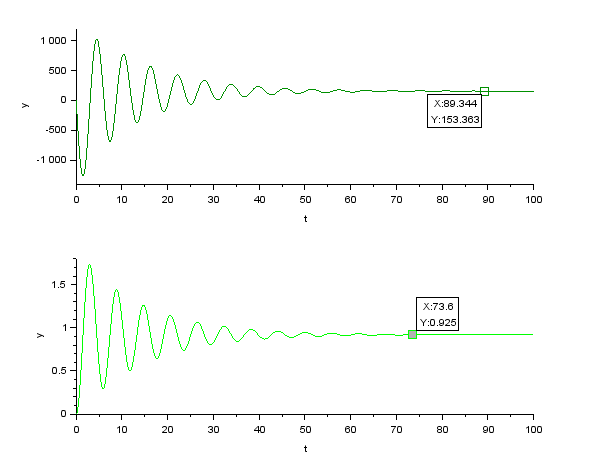
\includegraphics[width=\linewidth]{322.png}
	\caption{Переходные процессы $\omega\:  I$}\label{p322}
	\endminipage
\end{figure}

\subsection{Моделирование с различным моментом инерции нагрузки}
Ниже представлены переходные процессы:\\
\begin{enumerate}
	\item  $\alpha\:  U_y$ (рис \ref{p411}) и $\omega\:  I$ (рис \ref{p412})  при  $U=5\: J_l=0.5J_l=0.005kgm^2$
	\item  $\alpha\:  U_y$ (рис \ref{p421}) и $\omega\:  I$ (рис \ref{p422})  при  $U=5\: J_l=1.5J_l=0.015kgm^2$
\end{enumerate} 

\begin{figure}[H]
	\minipage{0.5\textwidth}
	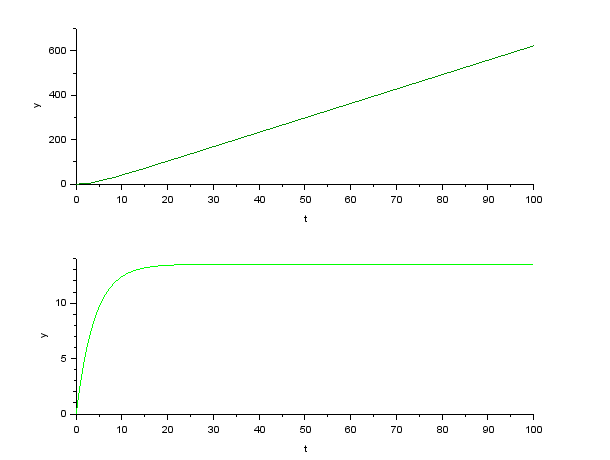
\includegraphics[width=\linewidth]{411.png}
	\caption{Переходные процессы $\alpha\:  U_y$}\label{p411}
	\endminipage\hfill
	\minipage{0.5\textwidth}
	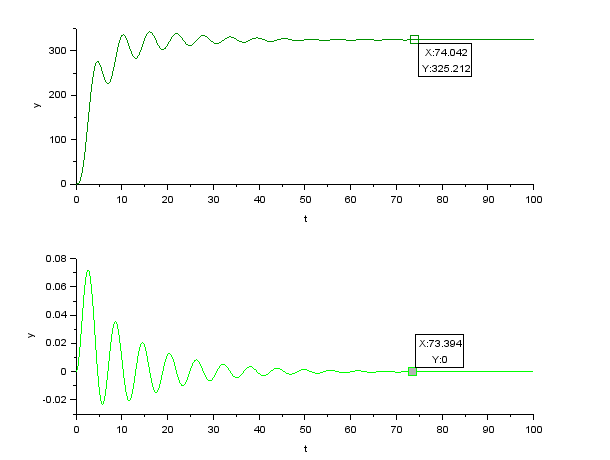
\includegraphics[width=\linewidth]{412.png}
	\caption{Переходные процессы $\omega\:  I$}\label{p412}
	\endminipage
\end{figure}
\begin{figure}[H]
	\minipage{0.5\textwidth}
	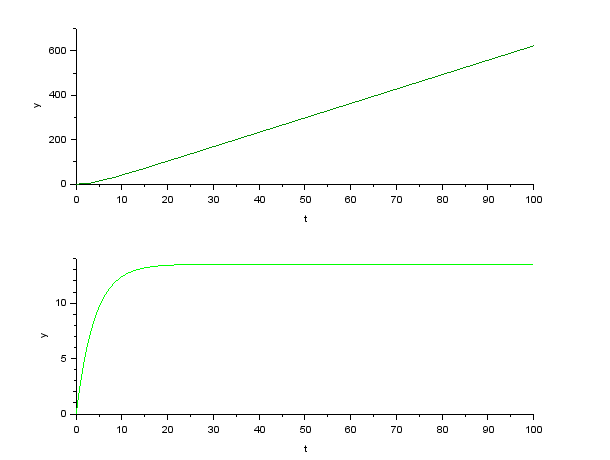
\includegraphics[width=\linewidth]{421.png}
	\caption{Переходные процессы $\alpha\:  U_y$}\label{p421}
	\endminipage\hfill
	\minipage{0.5\textwidth}
	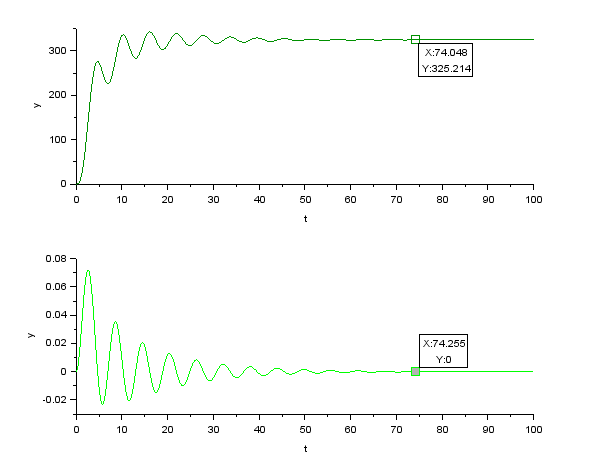
\includegraphics[width=\linewidth]{422.png}
	\caption{Переходные процессы $\omega\:  I$}\label{p422}
	\endminipage
\end{figure}

\subsection{Моделирование с различным передаточным отношением}
Ниже представлены переходные процессы:\\
\begin{enumerate}
	\item $\alpha\:  U_y$ (рис \ref{p511}) и $\omega\:  I$ (рис \ref{p512})  при  $U=5\: M_{sm}=0Nm\: i=1.75i=87.5$
	\item $\alpha\:  U_y$ (рис \ref{p521}) и $\omega\:  I$ (рис \ref{p522})  при  $U=5\: M_{sm}=0Nm\: i=0.75i=37.5$
	\item $\alpha\:  U_y$ (рис \ref{p531}) и $\omega\:  I$ (рис \ref{p532})  при  $U=5\: M_{sm}=300Nm\: i=1.75i=87.5$
	\item $\alpha\:  U_y$ (рис \ref{p541}) и $\omega\:  I$ (рис \ref{p542})  при  $U=5\: M_{sm}=300Nm\: i=1.75i=37.5$
\end{enumerate} 

\begin{figure}[H]
	\minipage{0.5\textwidth}
	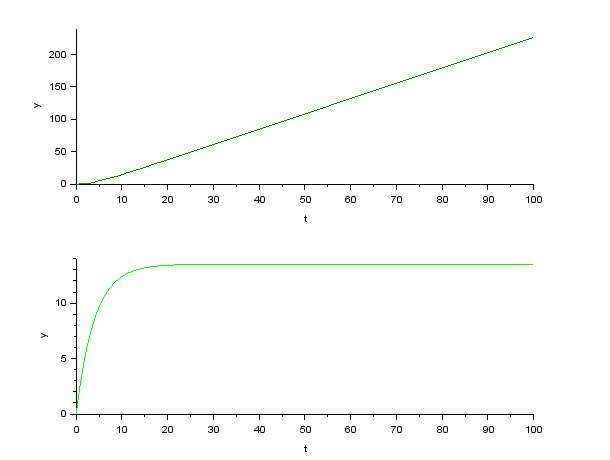
\includegraphics[width=\linewidth]{511.png}
	\caption{Переходные процессы $\alpha\:  U_y$}\label{p511}
	\endminipage\hfill
	\minipage{0.5\textwidth}
	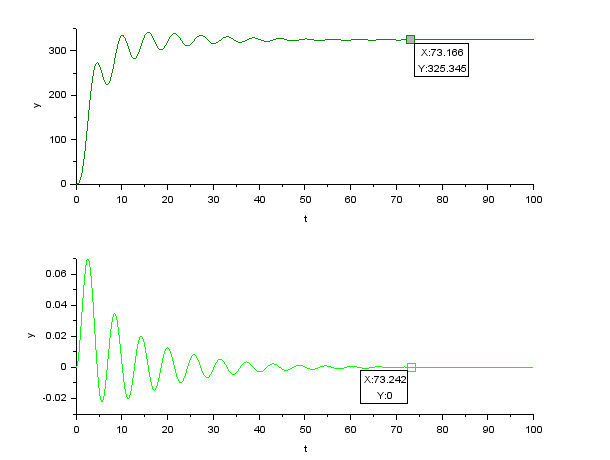
\includegraphics[width=\linewidth]{512.png}
	\caption{Переходные процессы $\omega\:  I$}\label{p512}
	\endminipage
\end{figure}
\begin{figure}[H]
	\minipage{0.5\textwidth}
	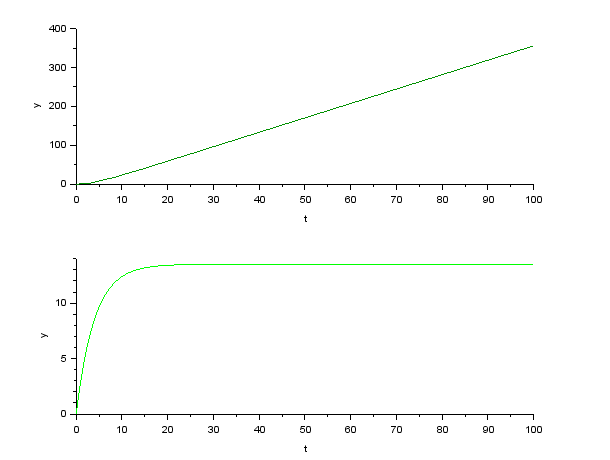
\includegraphics[width=\linewidth]{521.png}
	\caption{Переходные процессы $\alpha\:  U_y$}\label{p521}
	\endminipage\hfill
	\minipage{0.5\textwidth}
	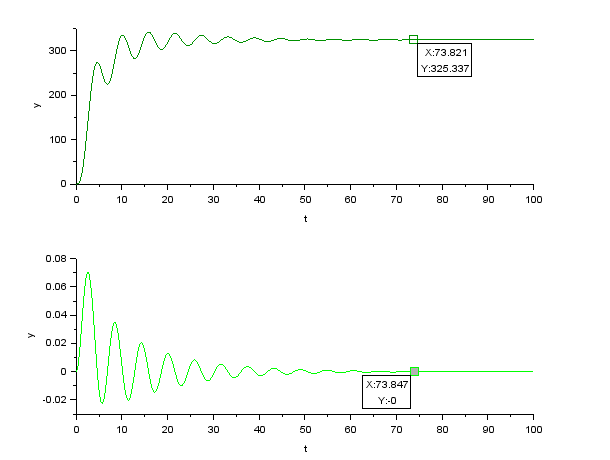
\includegraphics[width=\linewidth]{522.png}
	\caption{Переходные процессы $\omega\:  I$}\label{p522}
	\endminipage
\end{figure}
\begin{figure}[H]
	\minipage{0.5\textwidth}
	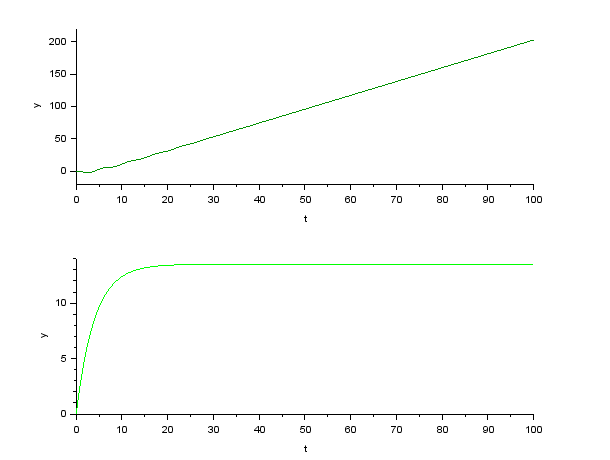
\includegraphics[width=\linewidth]{531.png}
	\caption{Переходные процессы $\alpha\:  U_y$}\label{p531}
	\endminipage\hfill
	\minipage{0.5\textwidth}
	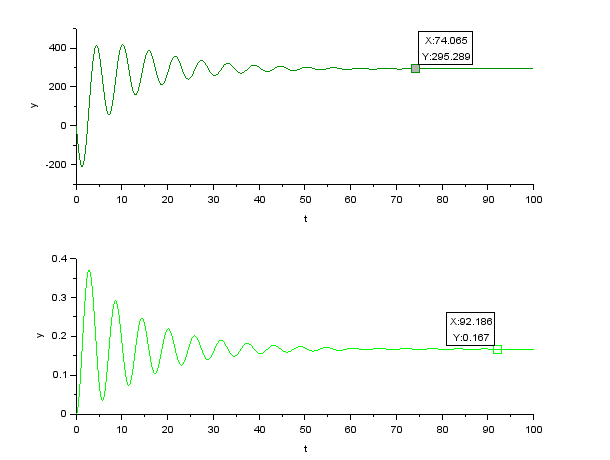
\includegraphics[width=\linewidth]{532.png}
	\caption{Переходные процессы $\omega\:  I$}\label{p532}
	\endminipage
\end{figure}
\begin{figure}[H]
	\minipage{0.5\textwidth}
	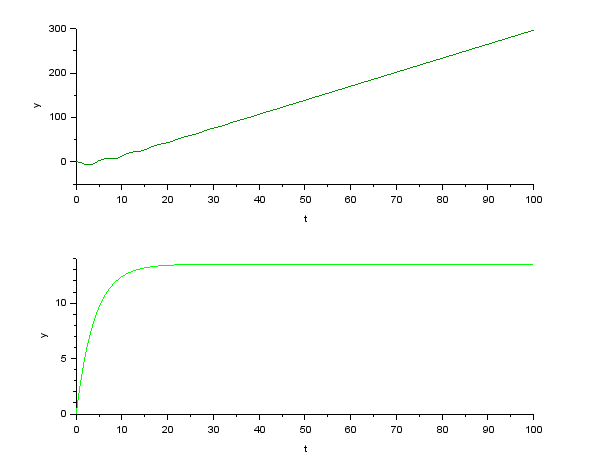
\includegraphics[width=\linewidth]{541.png}
	\caption{Переходные процессы $\alpha\:  U_y$}\label{p541}
	\endminipage\hfill
	\minipage{0.5\textwidth}
	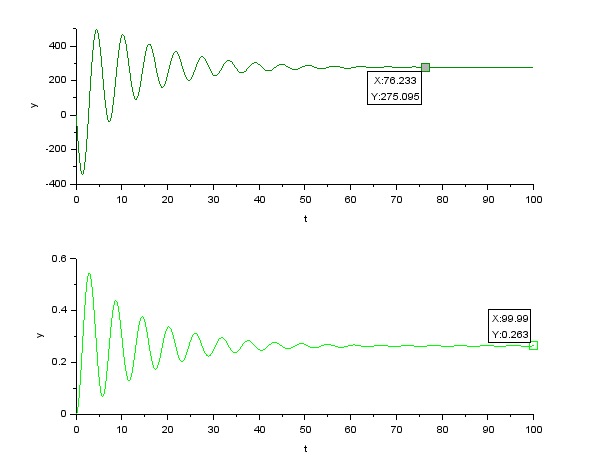
\includegraphics[width=\linewidth]{542.png}
	\caption{Переходные процессы $\omega\:  I$}\label{p542}
	\endminipage
\end{figure}

\subsection{Моделирование при меньших значениях постоянных времени}
Ниже представлены переходные процессы  $\alpha\:  U_y$ (рис \ref{p61}) и $\omega\:  I$ (рис \ref{p62})  при  $T_y=0.4ms\: T_a=0.7ms$.

\begin{figure}[H]
	\minipage{0.5\textwidth}
	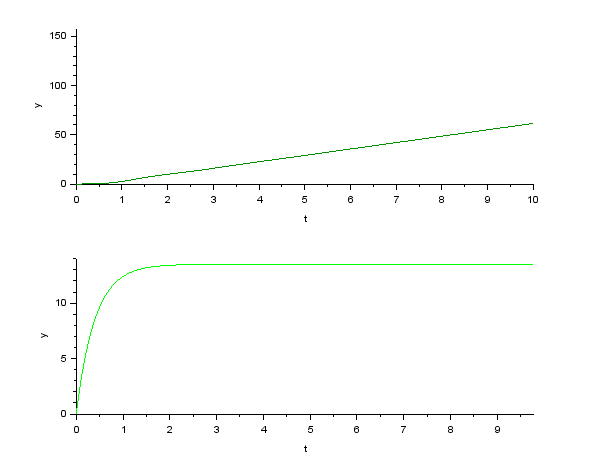
\includegraphics[width=\linewidth]{61.png}
	\caption{Переходные процессы $\alpha\:  U_y$}\label{p61}
	\endminipage\hfill
	\minipage{0.5\textwidth}
	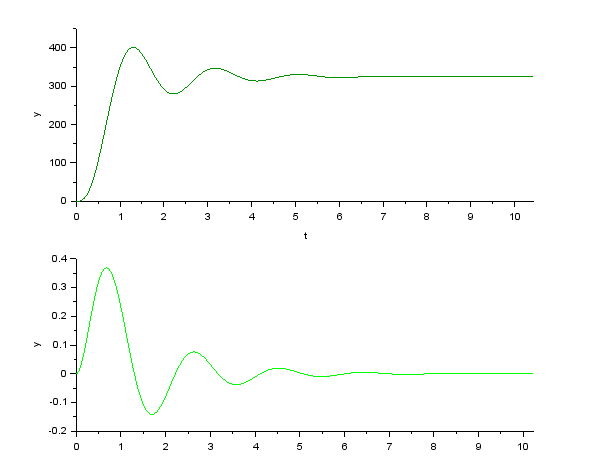
\includegraphics[width=\linewidth]{62.png}
	\caption{Переходные процессы $\omega\:  I$}\label{p62}
	\endminipage
\end{figure}

\subsection{Моделирование приближенной модели ЭМО}
Ниже представлены приближенная модель ЭМО (рис \ref{p7}) и переходные процессы  $\alpha_m\:  \omega_m$ (рис \ref{p72}) $M_{sm}=0\: U=5$.

\begin{figure}[H]
	\minipage{0.5\textwidth}
	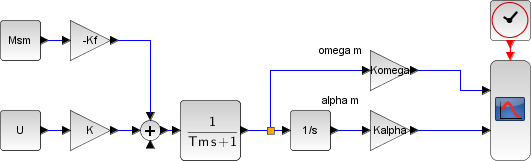
\includegraphics[width=\linewidth]{7.png}
	\caption{Приближенная модель ЭМО}\label{p7}
	\endminipage\hfill
	\minipage{0.5\textwidth}
	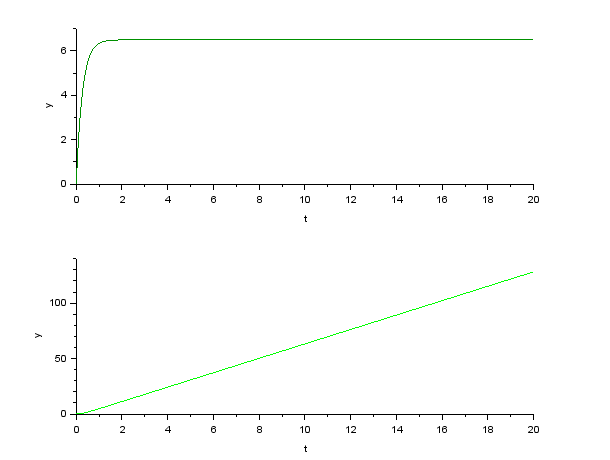
\includegraphics[width=\linewidth]{72.png}
	\caption{Переходные процессы  $\omega_m\: \alpha_m$}\label{p72}
	\endminipage
\end{figure}

\section{Вывод}
\begin{enumerate}
	\item В ходе данной работы были успешно созданы полная и приближенная модели ЭМО.
	\item Появление момента сопротивления увеличило $t_c\: \omega$ с 74с до 90с, при этом $\omega_c$(установившееся) уменьшилось с 325 рад/с до 239 рад/с, $I_c$ увеличилось с 0 до 0.5А. Коэффициенты затухания увеличились значительно, что заметно по графикам. Последующее увеличение момента сопротивления в два раза повлекло за собой уменьшение $omega_c$ и увеличение $I_c$ в 1.6 и 2 раза соотвественно.
	\item изменение момента инерции не повлекло за собой изменений переходных процессов.
	\item Изменение передаточного отношения при отсутствии момента сопротивления повлекло за собой рост $t_c$ угловой скорости и тока примерно на 0,8с. При наличии момента $t_c$ угловой скорости увеличился на 2.3с, а тока на 8с, при этом $omega_c$ уменьшилось на 20 рад/с, а $I_c$ увеличилось на 0.11A
	\item Уменьшение временных констант на порядок привело к уменьшению $t_c$ на порядок
	\item Из-за принятого упрощения в модели ЭМО переходный процесс $\omega_m$ практически теряет колебательный характер. 
\end{enumerate}

\end{document}